
\chapter{Lateness and Grouping Transform details}\label{apx:lateness}

\subsection{Watermarks}\label{sec:impl:dataflow:watermarks}

\todo{another diagram here illustrating the below (non-`graph', just showing multiple watermarks combining?)}

As mentioned in \cref{sec:prep:dataflow:when}, a \emph{watermark} is a heuristic indicating progress in the event stream.
There are several classes of watermark used in the Model.

Conceptually, each Collection in the system has a monotonic watermark in event time, called the \emph{global watermark}.
It approximates the point in time up to which the contents of the Collection have been produced.
It is not necessarily actually knowable or computable, either because of the properties of the Collection itself, or because of the distribution of the system amongst remote nodes.

Each Transform may consume (or produce) one or more Collections as inputs (outputs).
The minimum of the global watermarks of its input Collections is the Transform's \emph{global input watermark} ($\mathit{GIWM}$).
Similarly, the minimum of the global watermarks of its output Collections is its \emph{global output watermark} ($\mathit{GOWM}$).
In this way, I/O watermarks extend the notion carried by Collection watermarks to apply to the entire groups of streams Transforms consume and produce.

However, as mentioned above, global watermarks of Collections are not necessarily knowable.
Therefore, we introduce the concept of \emph{local watermarks}, which are scoped to each Transform Executor individually, and which provide us with the proxy through which to observe and control the system.

The \emph{local input watermark} ($\mathit{LIWM}$) of a Transform is a monotonically increasing lower bound on its global input watermark.
Similarly, the \emph{local output watermark} ($\mathit{LOWM}$) of a Transform is a monotonically increasing upper bound on its global output watermark.
This ensures that we always err on the side of treating data as non-late in cases of uncertainty (see \cref{sec:impl:dataflow:lateness}).

This also allows us to use the $\mathit{LOWM}$ of a Transform as the local watermark of a Collection it produces.
This means that each Transform receives a $\mathit{LIWM}$ which it cannot control, but can in turn specify its $\mathit{LOWM}$.
It can never (during normal operation\footnotemark) advance its $\mathit{LOWM}$ beyond its $\mathit{LIWM}$, because it cannot be sure that it won't receive input data which causes output late with respect to the new $\mathit{LOWM}$.

\footnotetext
{
The exceptions being a Transform at the edge of a watermark domain (\cref{sec:impl:dataflow:watermark-generation}) or watermarks being artificially advanced to the maximal timestamp in order to shut down a portion of the Pipeline.
} 

\begin{figure}[t]
	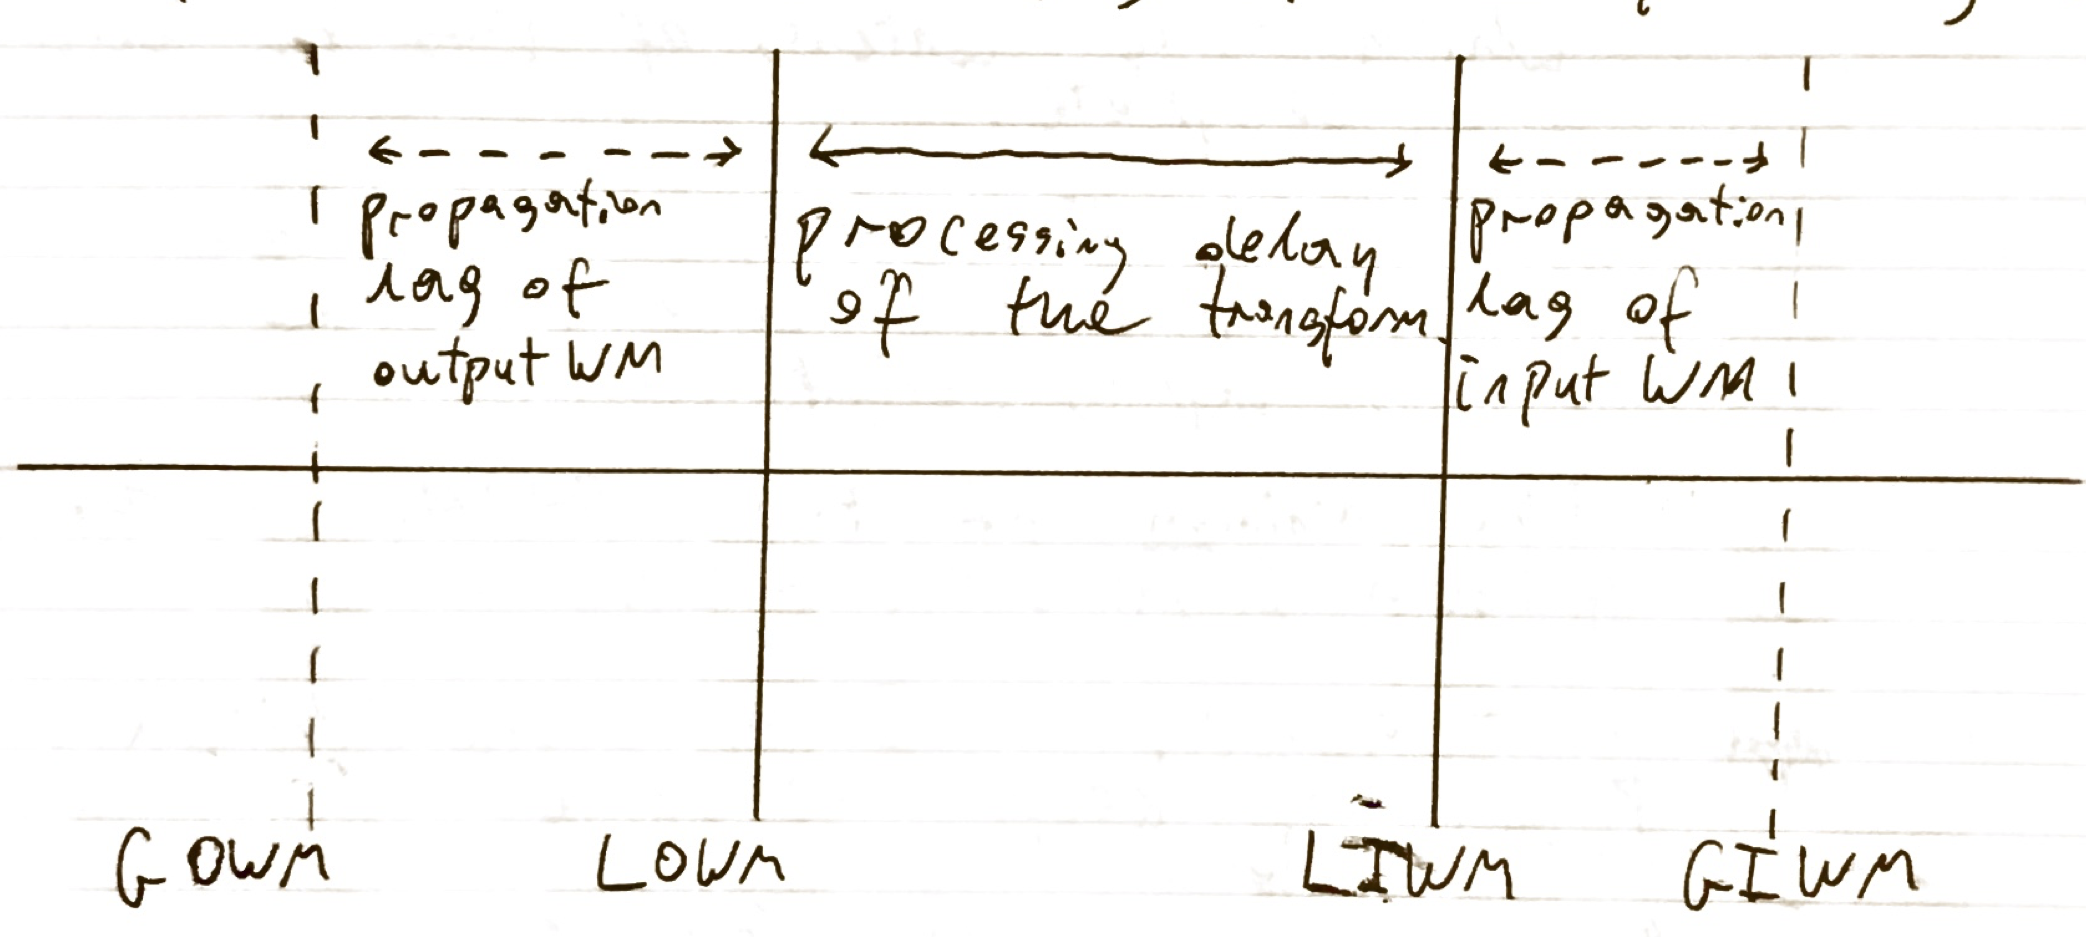
\includegraphics[width=\textwidth]{images/temp/lwm-transform-instantaneous}
	\caption{An instantaneous view of the watermarks of a particular Transform at a single point in processing time.}
	\label{fig:impl:lwm-instantaneous}
\end{figure}

We see that \[ \mathit{GOWM} \leq \mathit{LOWM} \leq \mathit{LIWM} \leq \mathit{GIWM} \] always holds for a particular Transform. \Cref{fig:impl:lwm-instantaneous} illustrates this.

We also distinguish a \emph{garbage-collection watermark}, which is a point in time beyond which it is safe to delete all state we hold about data.
It is usually a constant offset from the local input watermark.
It is not a true component of the Model, but rather an implementation detail necessary to avoid infinitely growing memory consumption.
This concept also limits the amount of lateness we can actually deal with in the system---elements behind the garbage-collection watermark are silently dropped.
However, the allowed lateness is tuneable, so that the user can choose between memory conservation and preservation of late data.

Watermarks provide us with a useful definition of \emph{doneness}.
In a system where unbounded data may or may not be present, it can be hard to determine when a particular section of the Pipeline is finished and will not receive or output any more data.
We therefore use the watermark to determine this; a watermark of maximal time (infinity) means that we will never receive / output data before that timestamp.
Since all time is before that timestamp, this implies that we will not receive or output any data at all, and hence we are done.
This is why bounded sources indicate they are done by simply advancing their watermark to the maximal timestamp.

\subsection{Lateness and its semantics}\label{sec:impl:dataflow:lateness}

The Model's robustness in dealing with unordered data is made possible by a comprehensive model of \emph{lateness}.

An element added to a Collection is \emph{late} if its timestamp is less than the global watermark of the Collection at the time of the addition, and \emph{non-late}\footnotemark\ otherwise.

\footnotetext
{
We use \emph{non-late} to avoid clashing with terms used to mark panes (\cref{sec:impl:dataflow:windows-panes}).
}

We say an element is \emph{droppable} when the the garbage collection watermark is after the end of the window to which it belongs; that is, the data is expired and may be dropped at any further point in the Pipeline.

A key invariant in the Dataflow Model which allows us to easily reason about the behaviour of our system is the following:

\todo{Implement invariant numbering and referencing. Temp labels inserted.}

\textbf{Inv 3A.: Only late input can result in lateness anywhere in the system.}

The goal of the system is to avoid lateness where possible, without holding back the progression of the Pipeline.
If we have an opportunity to integrate data which is technically late at one stage of the Pipeline into output which is non-late at the next, that is a good thing---it essentially takes advantage of the fact that the later part of a Pipeline may be progressing more slowly to allow data to catch up where possible, while also not holding the progress back to wait for potential late elements.

We can define a set of rules that Transforms in the Model must follow which ensure that the above invariant holds.

A complication arises because we only have access to local watermarks, which are mere approximations of the global watermark, in order to do this.
\Cref{fig:impl:lateness-knowability} illustrates the knowability of whether input or output data is late or not, from the perspective of an individual Transform.

\begin{figure}[t]
	\subfloat[][The knowability of the lateness of $t_{\mathit{in}}$ with respect to the $\mathit{LIWM}$.]{
		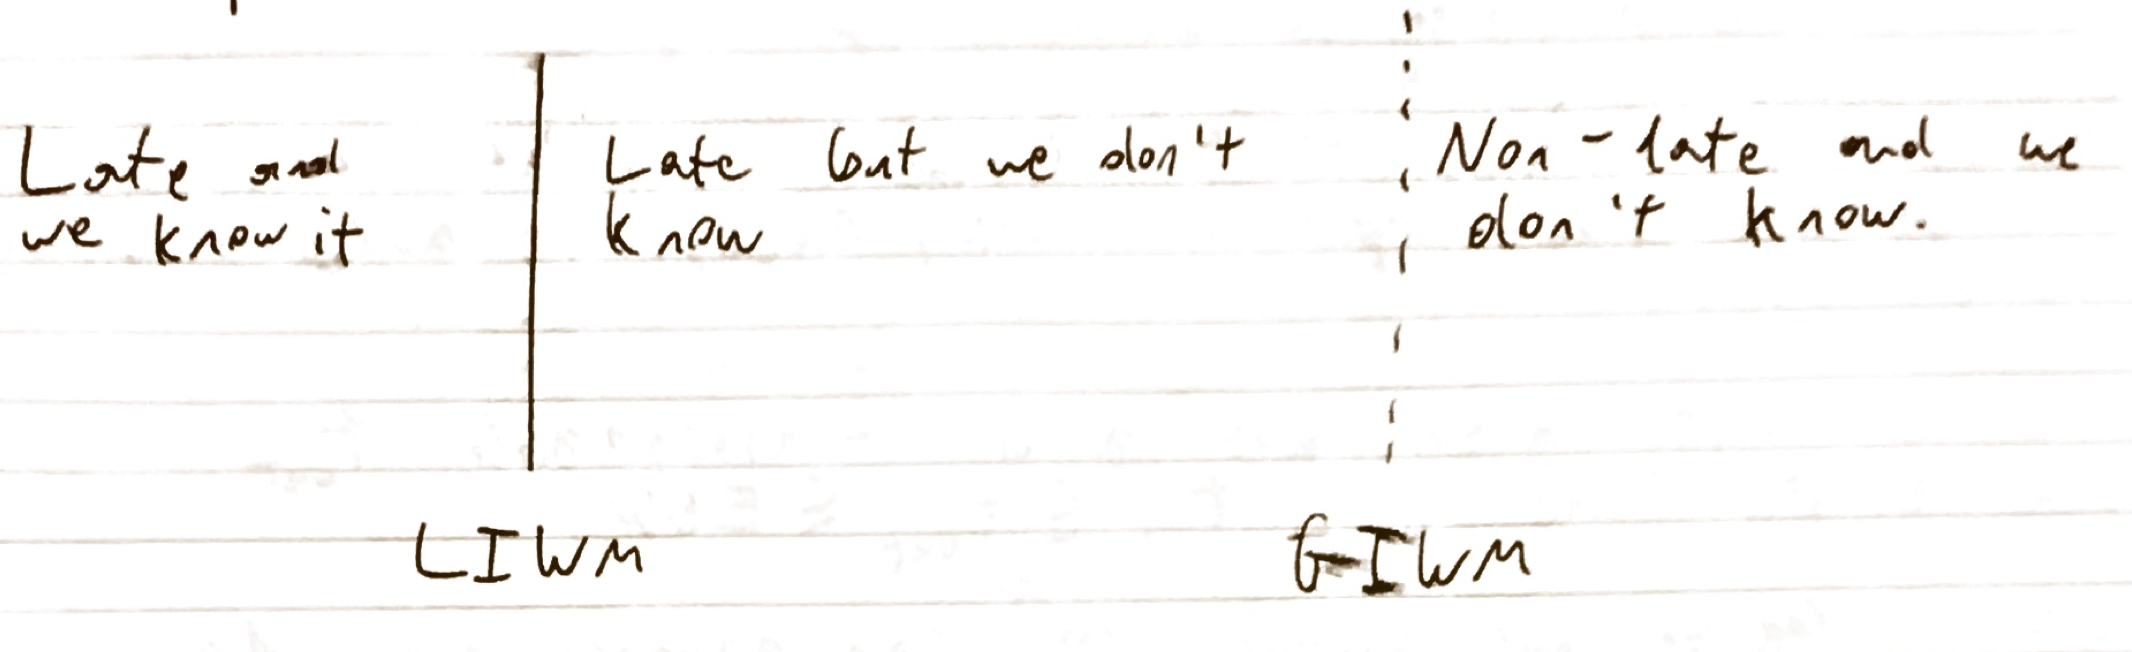
\includegraphics[width=\textwidth]{images/temp/lateness-knowability-input}
	}\\
	\subfloat[][The knowability of the lateness of $t_{\mathit{out}}$ with respect to the $\mathit{LOWM}$.]{
		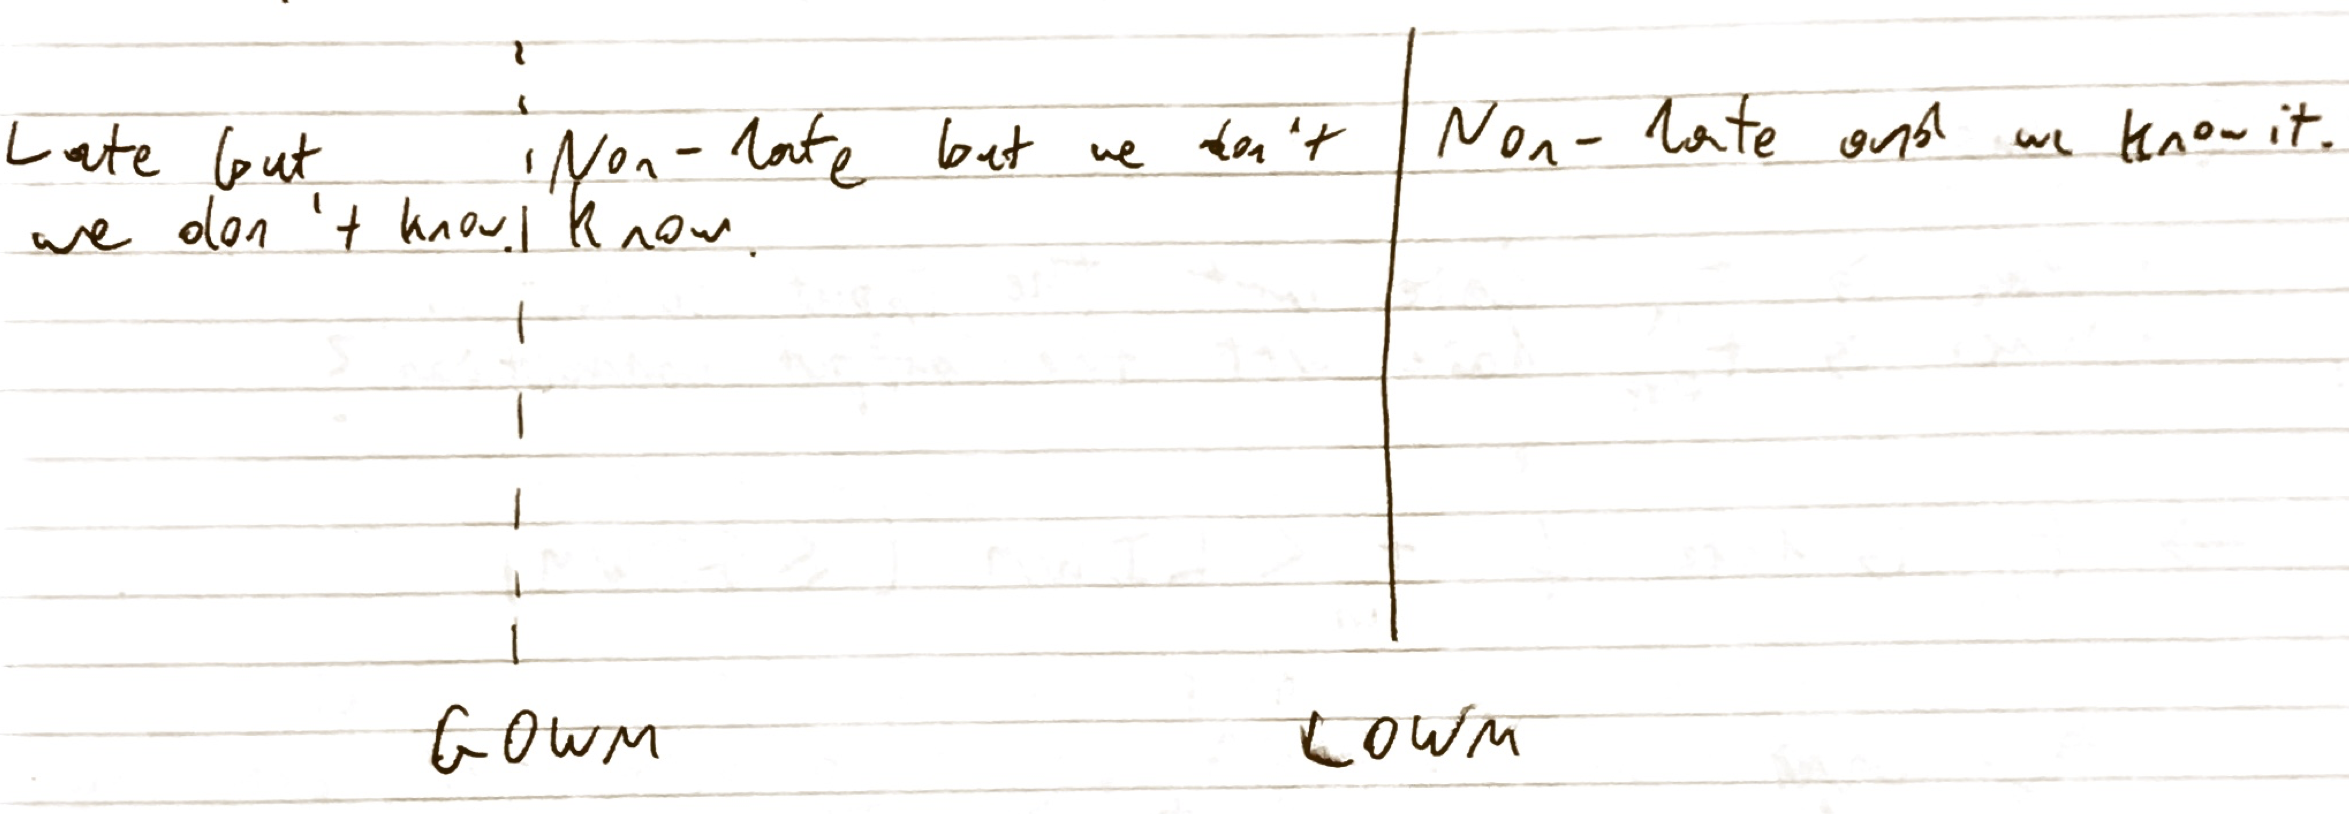
\includegraphics[width=\textwidth]{images/temp/lateness-knowability-output}
	}
	\caption{Diagram illustrating the knowability of the lateness of elements with respect to their position relative to local watermarks.}
	\label{fig:impl:lateness-knowability}
\end{figure}


We therefore expand the original invariants to the following, which ensure the original invariant it is maintained in the situation of imprecise knowledge of the true watermark.

\todo{do we need some sort of informal proof that these actually ensure the original one?}


\begin{itemize}
	\item \textbf{3B(i).: If an element is added to an input Collection non-late, output derived from that element must be added to its respective Collection non-late.}
	\item \textbf{3B(ii).: If an element is added to an input Collection non-droppable, then output derived from that element must be added to its Collection non-droppable.}
	\item \textbf{3B(iii).: If a pane is emitted, it should not be droppable.}
	\item\textbf{ 3B(iv).: The panes of a window must follow the sequence} \verb|EARLY* ON_TIME? LATE*| \textbf{(zero or more early panes, then zero or one on-time panes, then zero or more late panes).}
	\item \textbf{3B(v).: If a pane is marked early or on-time, it must be non-late in actuality.}
	\item \textbf{3B(vi).: If a pane is marked late, it must have been derived \emph{exclusively} from late input elements.}
\end{itemize}

\subsection{Grouping Transform semantics}\label{sec:impl:dataflow:grouping}

\todo{this section needs rewritten to use much more diagrams, tables and code and less prose.}

Keeping in mind that the overall goal is to allow the output watermark to progress as fast as possible without introducing any lateness which was not introduced at the source, an overview of the algorithm every Grouping Transform must follow can be defined.

Suppose that we have received an element with timestamp $t_{\mathit{in}}$ which belongs to a particular window $w$ with inclusive upper bound $t_{\mathit{EOW}}$, and it is abut to be buffered for output at a later stage.
The element also has a time $t_{\mathit{out}}$, from which the timestamp of the pane this element will be part of is derived.\footnotemark\ 
This time is such that \[t_{\mathit{in}} \leq t_{\mathit{out}} \leq t_{\mathit{EOW}}\] and is included to allow the advancement of the output watermark even if the current window is not yet ready for output.

\footnotetext
{
Both $t_{\mathit{out}}$ and the derived pane timestamp are controlled by a user-specifiable OutputTimeFn, though in most cases the default of `use the end-of-window time for both' is used.
}

For example, with sliding windows, once we are in the context of one particular window (elements can have multiple windows) it is safe to treat the timestamp of an element as the end of the window, because all elements in the window are processed the same and the difference is not observable in the output.
Doing this, however, will allow us to advance the watermark to just before the end of the current window (and new elements in this window will not be late, since we perform the lateness checks on $t_{\mathit{out}}$), allowing earlier sliding windows to close and output their panes with less delay.

We don't want elements that will be output late anyway to hold up the output watermark, except to avoid becoming droppable.

\todo{actually reference back to numbered invariants.}

\subsubsection{Lateness}

\begin{figure}
	\centering
	\subfloat[][If $t_{\mathit{in}}$ could be non-late, then $t_{\mathit{out}}$ must be non-late. Similarly, if $t_{\mathit{out}}$ could be late, then $t_{\mathit{in}}$ must be late. If $t_{\mathit{out}}$ is non-late and the $\mathit{LIWM}$ has not reached the end-of-window, $t_{\mathit{out}}$ is on-time.]{
		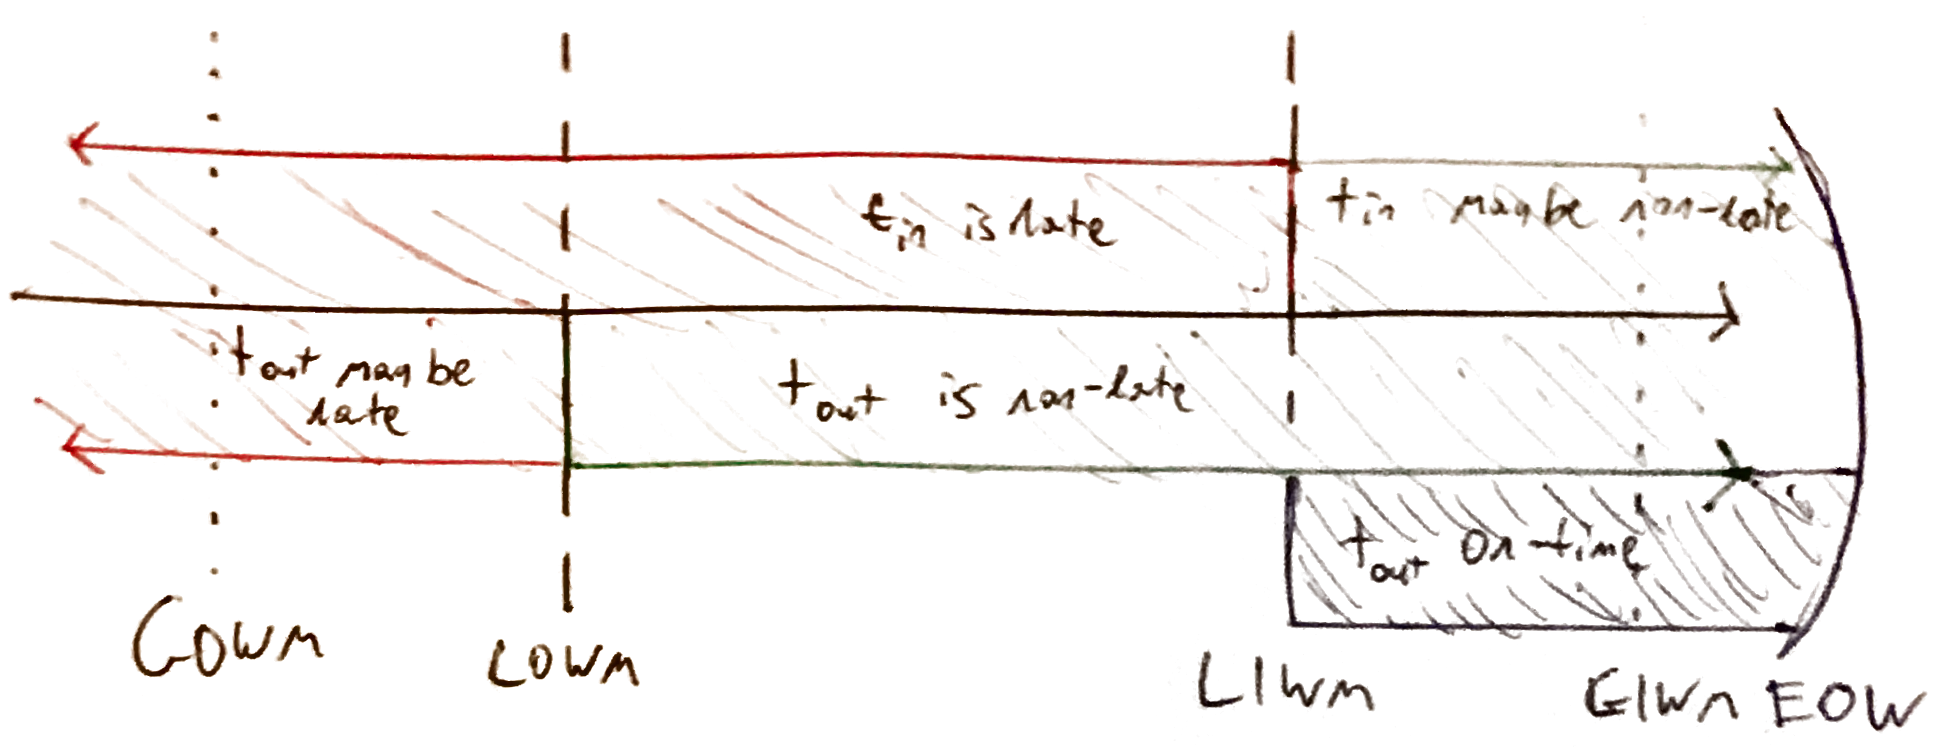
\includegraphics[width=\textwidth]{images/temp/lateness-semantics-1}
		\label{fig:impl:lateness-semantics:a}
	}\\
	\subfloat[][If the $\mathit{LIWM}$ has passed the end-of-window, then $t_{\mathit{in}}$ is definitely late. $t_{\mathit{out}}$ may technically be non-late, but it is not on-time.]{
		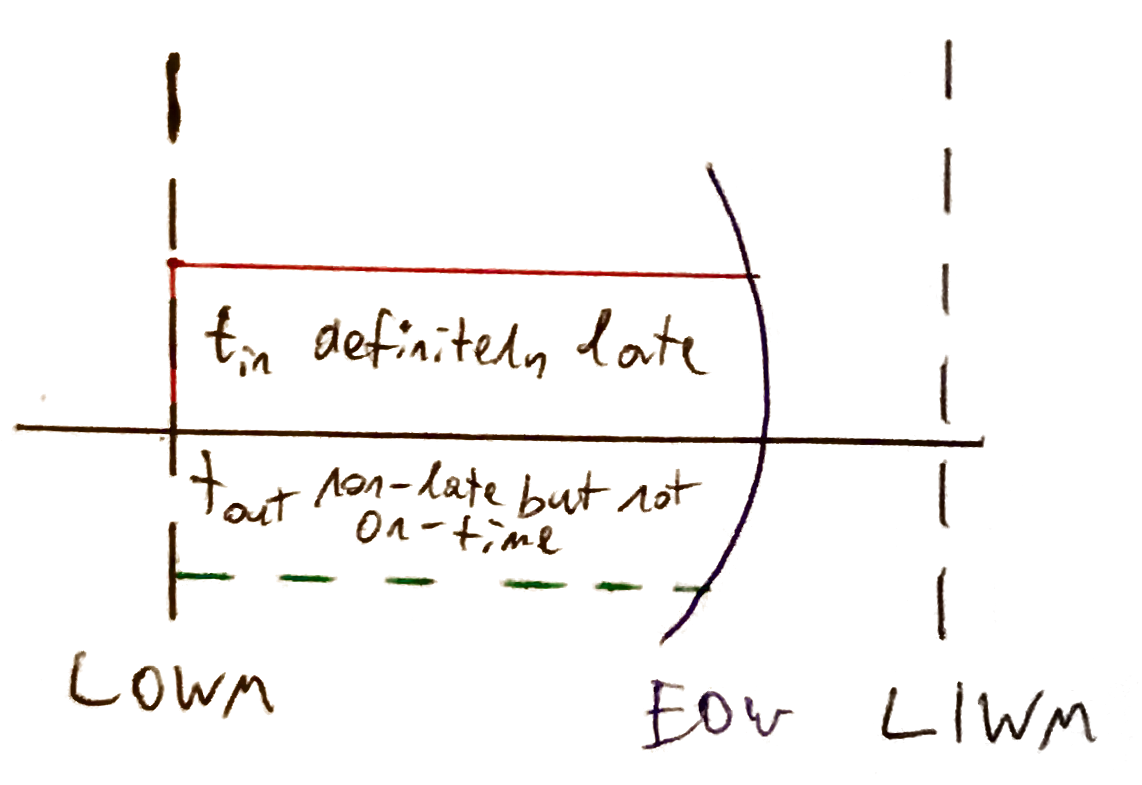
\includegraphics[width=0.5\textwidth]{images/temp/lateness-semantics-2}
	}
	\caption{Diagrams showing regions in event time associated with particular late/non-late or on-time knowledge of $t_{\mathit{in}}$ and $t_{\mathit{out}}$.}
	\label{fig:impl:lateness-semantics}
\end{figure}

There are two questions to answer in order to proceed:
\begin{enumerate}
	\item When is $t_{\mathit{in}}$ late with regards to the input Collection?
	\item When is $t_{\mathit{out}}$ late with regards to the output Collection?
\end{enumerate}

Referring to \cref{fig:impl:lateness-semantics}\subref{fig:impl:lateness-semantics:a} we see that
\begin{enumerate}
	\item \begin{itemize}
	\item $t_{\mathit{in}}$ \textbf{is late} if $t_{\mathit{in}} < \mathit{LIWM}$.
	\item Otherwise, if $t_{\mathit{in}} \geq \mathit{LOWM}$, $t_{\mathit{in}}$ \textbf{could be late} (but we don't know).
	\end{itemize}
	\item \begin{itemize}
	\item $t_{\mathit{out}}$ \textbf{is non-late} if $t_{\mathit{out}} \geq \mathit{LOWM}$.
	\item Otherwise, if $t_{\mathit{out}} < \mathit{LOWM}$, $t_{\mathit{out}}$ \textbf{could be late}. However, in this case, $t_{\mathit{in}}$ \textbf{is definitely late} since $t_{\mathit{in}} \leq t_{\mathit{out}} < \mathit{LOWM} \leq \mathit{LIWM}$.
	\end{itemize}
\end{enumerate}

Note that when $t_{\mathit{in}}$ is late, but $t_{\mathit{out}}$ is non-late, and also $\mathit{LIWM} \leq t_{\mathit{EOW}}$, it is valid with respect to our invariants to treat $t_{\mathit{out}}$ as either late or non-late.
We revisit this choice later.

We have a further requirement for the behaviour of our grouping Transform.
We want to be sure to fire at most one on-time pane.
It \textbf{must} contain all non-late input data up to the end of the window.
It could also contain some late input data which luckily arrived before we emitted the pane (but we do not wait for such data).

To allow us to reason about this, we say that $t_{\mathit{out}}$ is \emph{on-time} if it is non-late, and the input watermark has not yet advanced past its $t_{\mathit{EOW}}$, that is the element arrived early enough to be included in the on-time pane.

\subsubsection{Droppability}

We need to determine two further pieces of information:
\begin{enumerate}
	\item When is the input element droppable?
	\item When is the resulting output going to be droppable?
\end{enumerate}

Denote the allowed lateness used to determine the garbage collection watermark as $\delta$.

$t_{\mathit{in}}$ \textbf{is droppable} if $t_{\mathit{EOW}} < (\mathit{LIWM} - \delta)$.\\
$t_{\mathit{in}}$ \textbf{could be non-droppable} if $t_{\mathit{EOW}} \geq (\mathit{LIWM} - \delta)$.\\
$t_{\mathit{out}}$ \textbf{is non-droppable} if $t_{\mathit{EOW}} \geq (\mathit{LOWM} - \delta)$.\\
$t_{\mathit{out}}$ \textbf{could be droppable} if $t_{\mathit{EOW}} < (\mathit{LOWM} - \delta)$.

Now, if $t_{\mathit{in}}$ \textbf{could be non-droppable} then $t_{\mathit{out}}$ \textbf{is} non-droppable, since \[(\mathit{LOWM} - \delta) \leq (\mathit{LIWM} - \delta) \leq t_{\mathit{in}} \leq t_{\mathit{out}}\;\text{.}\]
Also, if $t_{\mathit{out}}$ \textbf{could be droppable} then $t_{\mathit{in}}$ \textbf{is} droppable, since \[t_{\mathit{in}} \leq t_{\mathit{out}} \leq (\mathit{LOWM} - \delta) \leq (\mathit{LIWM} - \delta)\;\text{.}\]

\todo{mention all Grouping Transform computation is per window per key}

\subsubsection{Transform behaviour}

A Grouping Transform does not output panes on receiving input elements, but only when it is triggered.
It can, however, modify its output watermark on receiving elements, and managing this well is crucial to achieve good progress in the Pipeline.

The priorities adopted are:
\begin{itemize}
	\item if it is possible to output data non-late, do that as much as we can;
	\item (TODO go back and find out what this was meant to mean) if process late data and may output late, hold the local output watermark as little as possible (allow it to progress as far as possible);
	\item (TODO introduce this as invariant 3C) ensure that the invariants hold and that only a single on-time pane is output.
\end{itemize}

We introduce yet another timestamp for each element, the emission timestamp $t_{\mathit{emit}}$.
It is the timestamp that we actually input into the combination function of the OutputTimeFn to obtain the final timestamp of the resultant pane $T_{\mathit{emit}}$.
This additional transformation affords us the flexibility to combine late data with non-late data to obtain a non-late result.
We require that $t_{\mathit{out}} \leq t_{\mathit{emit}} \leq t_{\mathit{EOW}} + \delta$ where $\delta$ is the allowed lateness.

On receiving each element, then, the Transform Executor must decide:
\begin{itemize}
	\item should the element be dropped?
	\item what hold should be placed on the local output watermark? (see remark above)
	\item what value will be used for $t_{\mathit{emit}}$?
\end{itemize}

\todo{the below cases will translate well to a code listing}

\textbf{Case 0: $t_{\mathit{EOW}} < (\mathit{LIWM} - \delta)$}\\
Drop the element.
Since $t_{\mathit{in}}$ and $t_{\mathit{out}}$ are both within the window, they are both certainly droppable and therefore so is the element.

\textbf{Case 1: $t_{\mathit{out}}$ is on-time}\\
We treat the element as non-late.
We set $t_{\mathit{emit}} \coloneq t_{\mathit{out}}$ and place a hold at $t_{\mathit{out}}$.

\textbf{Case 2: $t_{\mathit{out}}$ is not on-time}\\
This is either because $t_{\mathit{out}}$ is possibly late, or because the on-time pane may have already fired.
In either case, $t_{\mathit{in}}$ is definitely late.

We set $t_{\mathit{emit}} \coloneq t_{\mathit{EOW}}$, attempting to shift the element forward in order to possibly include it in an on-time pane.
We could also use the current output watermark for $t_{\mathit{emit}}$, but this would have the effect of significantly holding back watermark progress.
The watermark hold logic described above ensures that the hold is set at $t_{\mathit{EOW}} + \delta$, ensuring we won't produce a droppable pane.

\todo{diagram}

\Cref{fig:todo} illustrates the two situations that are possible in this case. It can be seen that $t_{\mathit{emit}}$ will, in general, be late once emitted, but never be droppable. 
The timestamp used is the latest for the correct window, and the hold used is the latest that prevents dropping.
In this way we allow the watermark to progress in the presence of late data, while ensuring it doesn't become droppable in the process.

\subsubsection{Labelling panes}

When a Grouping Transform Executor is triggered and outputs a pane (again, simply an element of the output Collection), it must label it as either \verb|EARLY|, \verb|ON_TIME| or \verb|LATE|.
The pane is also itself an element, and will be either late or non-late.
This is orthogonal to its label, which merely states whether the pane represents only a subset of non-late data in a window (\verb|EARLY|), all of the non-late data (\verb|ON_TIME|), or only late data (\verb|LATE|).

The decision is made based on the state of the watermarks and $T_{\mathit{emit}}$, the combined output timestamp determined by the OutputTimeFn from all individual $t_{\mathit{emit}}$ values.
It also determines whether a pane is \emph{final}, which lets the downstream know that no more panes for this window will be emitted (as they would have been emitted droppable).

\todo{replace below with code listing}

Therefore if $T_{\mathit{emit}} \geq \mathit{LOWM}$, it is non-late.
By design, every $t_{\mathit{out}}$ that went into the pane was non-late as well.

If $T_{\mathit{emit}} < \mathit{LOWM}$, it is possibly late (it could be on either side of the $\mathit{GOWM}$).
By design, this means that at least some of the $t_{\mathit{out}}$ were treated as late, meaning the corresponding $t_{\mathit{in}}$ were certainly late.
In this case, it is appropriate to output this pane element late and label it late if we need to.

The pane can be marked on-time if $T_{\mathit{emit}}$ is non-late, and if $\mathit{LIWM} > EOW$.
This is because any elements which come in after this condition holds will be treated as late, meaning that they do not need to be included in the on-time pane.
They may still be included in this pane if they arrive before we output it, but we do not have to wait for them, since they were produced late to begin with.

The pane is marked final if $\mathit{LIWM} - \delta > t_{\mathit{EOW}}$, since any incoming elements after this condition starts to hold will just be dropped.

Therefore the pane is labelled as follows:
\begin{itemize}
	\item If $T_{\mathit{emit}}$ is possibly late, label it late.
	\item If $T_{\mathit{emit}}$ is non-late, label it on-time is possible, and early otherwise.
	\item Additionally, label the pane as final if appropriate.
\end{itemize}

\subsubsection{OutputTimeFn}
Grouping Transforms aggregate element data into an output value.
They must also aggregate the elements' timestamps into a single timestamp used for the output pane.
This concern is often orthogonal to the type of data transformation being performed, and so the Model allows its specification orthogonally, through the use of \verb|OutputTimeFn|s.

An \verb|OutputTimeFn| specifies three aspects of the aggregation:
\begin{enumerate}
	\item how $t_{\mathit{in}}$ maps to $t_{\mathit{out}}$;
	\item how multiple $t_{\mathit{emit}}$ timestamps combine to give the pane timestamp $T_{\mathit{emit}}$;
	\item how multiple tentative $T_{\mathit{emit}}$ values are combined when two windows merge.
\end{enumerate}

There are several options available for these, but in the vast majority of cases $t_{\mathit{out}}$ is set to $t_{\mathit{EOW}}$, making the other two aspects trivial.
